%\begin{figure}
%	\centering
%   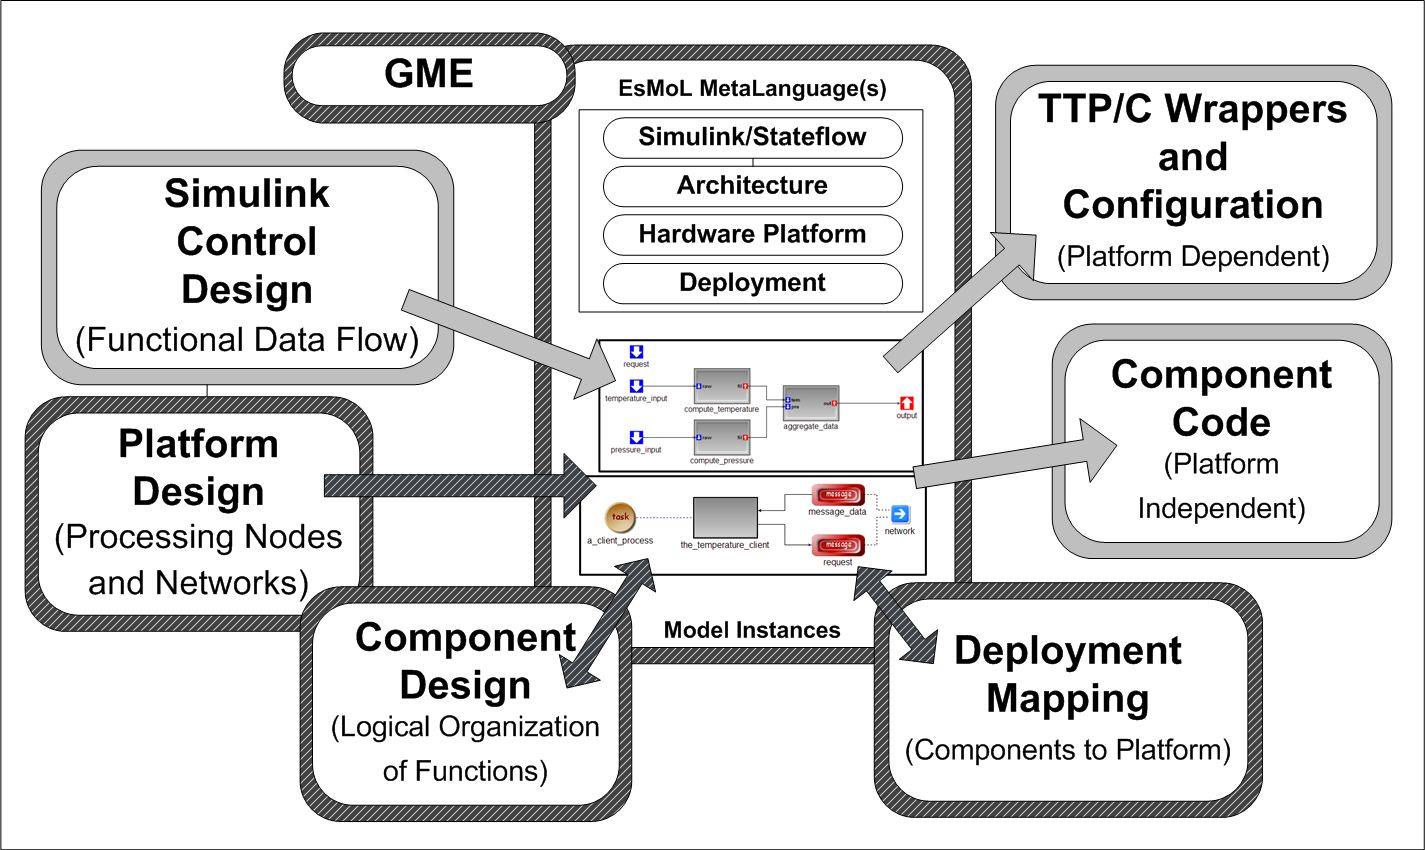
\includegraphics[width=0.55\columnwidth]{diagrams/usecase1.png}
%   \caption{Stage 1. Model interpreters automatically import Simulink and Stateflow control designs and synthesize code. Users directly enter and edit platform models, design software architecture, and create deployments using the Generic Modeling Environment (GME).}
%   \label{fig:uc1}
%\end{figure}

%Fig. \ref{fig:uc1} shows the tool flow for the existing tool chain.  
Control designs in Simulink are integrated using a graphical modeling language describing software architecture.  Components within the architecture are assigned to tasks, which run on nodes in the platform.  

\subsection{Integration Details}

\begin{figure}
	\centering
	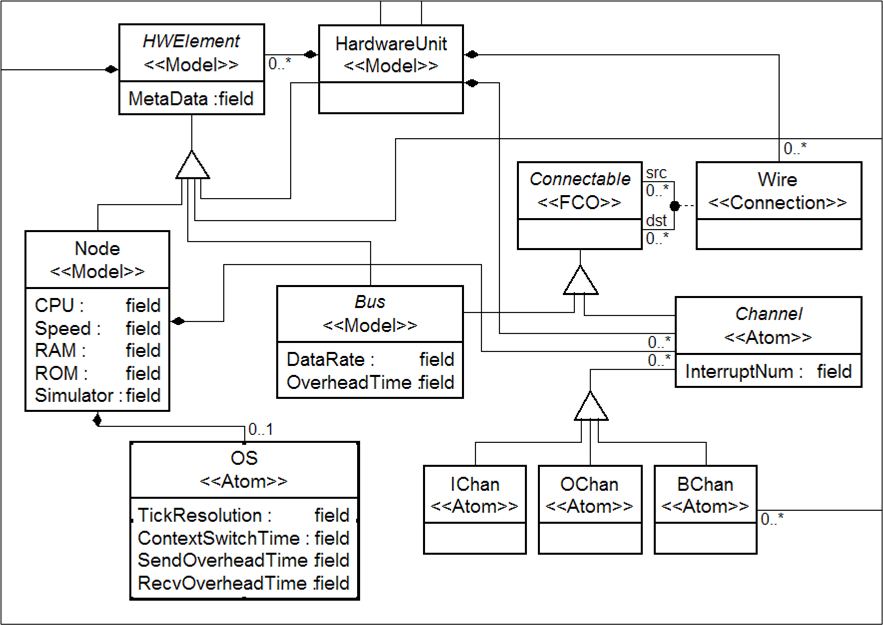
\includegraphics[width=0.75\columnwidth]{diagrams/platform.png}
	\caption{Platforms. This metamodel describes a simple language for modeling the topology of a time-triggered processing network.  A sample platform model is included.}
	\label{fig:platform}
\end{figure}

The Simulink and Stateflow sublanguages of our modeling environment are described elsewhere, though the ESMoL language changes many of the other design concepts from older languages described by Neema~\cite{KS:ISIS-04-505}.

In our toolchain we created a number of code generators. In the construction of the two main platform-independent code generators (one for Simulink-style models and another one for Stateflow-style models), we have used a higher-level approach based on graph transformations \cite{isis:great}. This approach relies on an assumption that (1) models are typed and attributed graphs with specific structure (governed by the metamodel of the language) and (2) executable code can be produced as an abstract syntax graph (which is then printed directly into source code). This graph transformation-based approach allows a higher-level representation of the translation process, which lends itself to algorithmic analysis of the transformations.

\begin{figure}
	\centering
	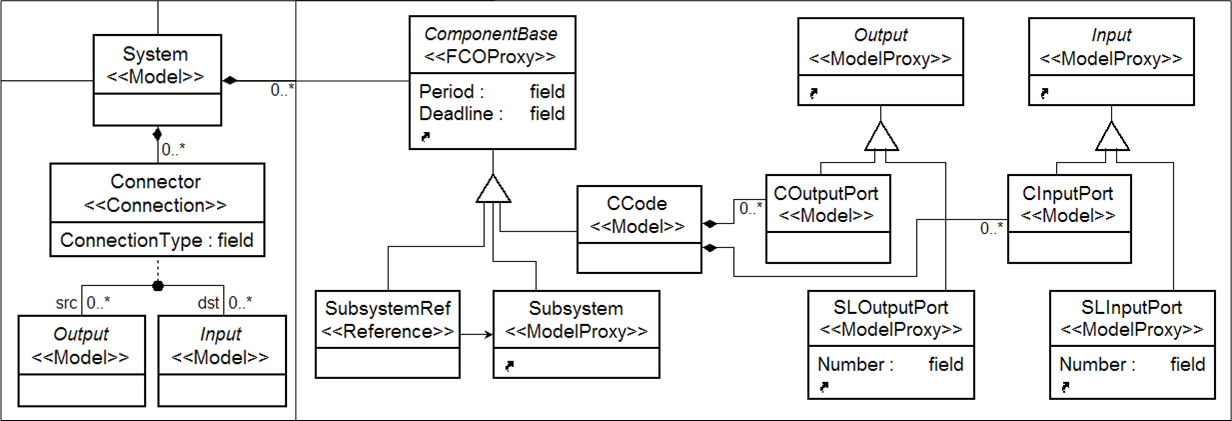
\includegraphics[width=0.9\columnwidth]{diagrams/arch_lang.png}
	\caption{Architecture Metamodel. Architecture models use Simulink subsystems or C code functions as components, adding attributes for real-time execution. The Input and Output port classes are typed according to the implementation class to which they belong.}
	\label{fig:arch}
\end{figure}

The models in the example, and the metamodels described in the sequel were created using the ISIS Generic Modeling Environment tool (GME)~\cite{isis:gme}.  GME allows language designers to create stereotyped UML-style class diagrams defining metamodels.  The metamodels are instantiated into a graphical language, and metamodel class stereotypes and attributes determine how the elements are presented and used by modelers.  The GME metamodeling syntax may not be entirely familiar to the reader, but it is well-documented elsewhere~\cite{karsai:mic}. Class concepts such as inheritance can be read analogously to UML.  Class aggregation represents containment in the modeling environment, though an aggregate element can be flagged as a port object.  In the modeling environment a port object will also be visible at the next higher level in the model hierarchy, and available for connections.  The dot between the Connectable class and the Wire class represents a line-style connector in the modeling environment.

High-confidence systems require platforms that provide services and guarantees for needed properties, e.g. fault containment, temporal firewalls, etc. These critical services (like partitioning) should be provided by the platform and not re-implemented from scratch by system developers~\cite{alberto:2002}.  Note that the platform also defines a 'Model of Computation' \cite{Lee:M97/11}. An MoC governs how the concurrent objects of an application interact (i.e. synchronization and communication), and how these activities unfold in time. The simple platform definition language shown in Fig. \ref{fig:platform} contains relationships and attributes for describing a time-triggered network. 

\begin{figure}
	\centering
%	\subfigure[Tasks contain Components and associate with Nodes.]{
	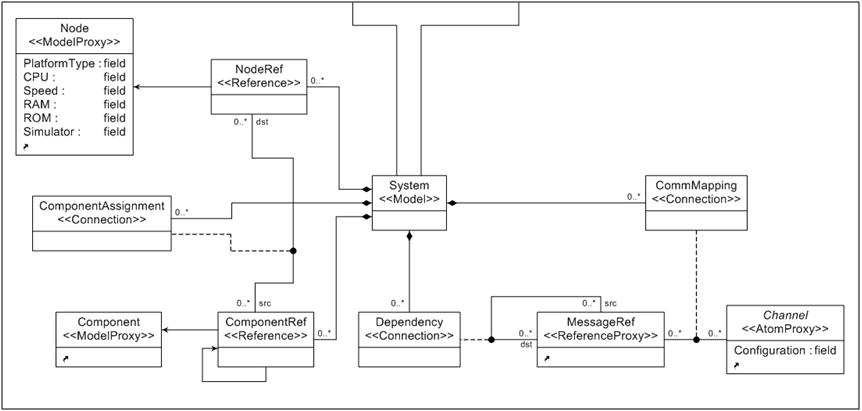
\includegraphics[width=\columnwidth]{diagrams/depnew.png}
%	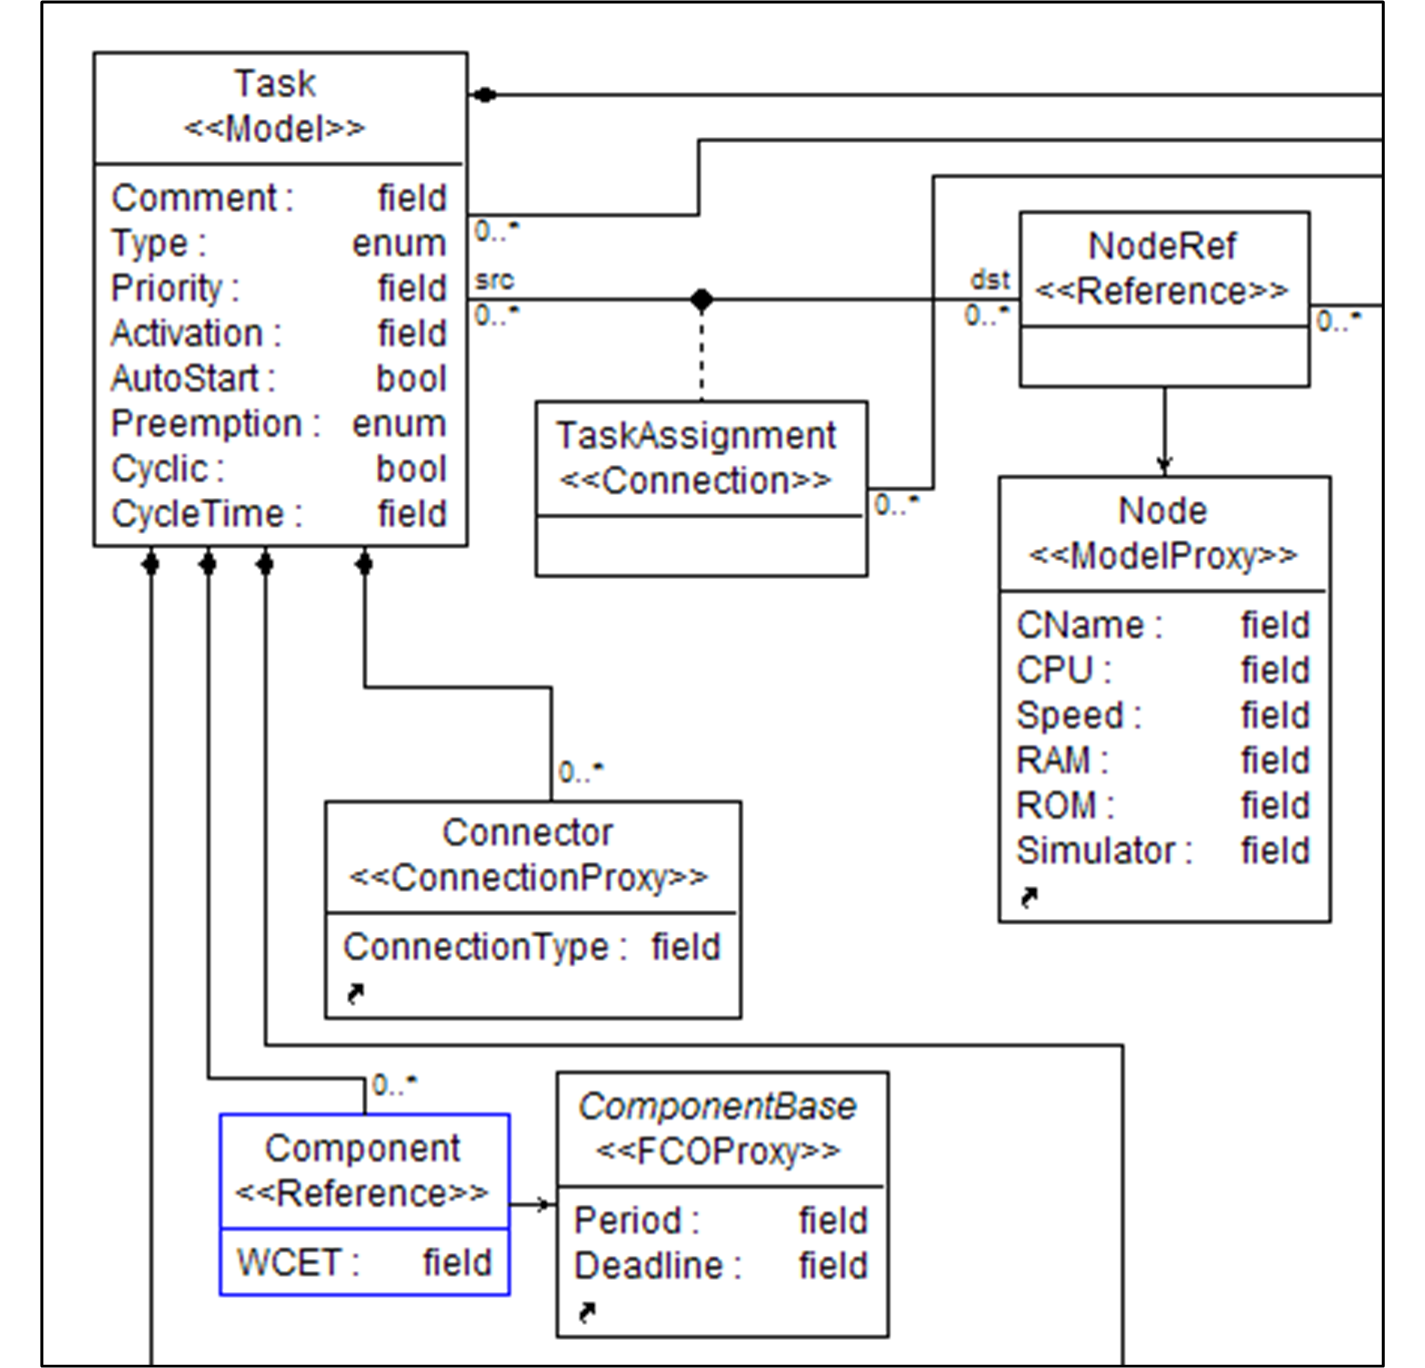
\includegraphics[scale=1]{diagrams/depcompnew.png}
%	\label{fig:depcomp}
%	}
%	
%	\subfigure[InputPorts and OutputPorts from Simulink connect to Messages.]{
%	%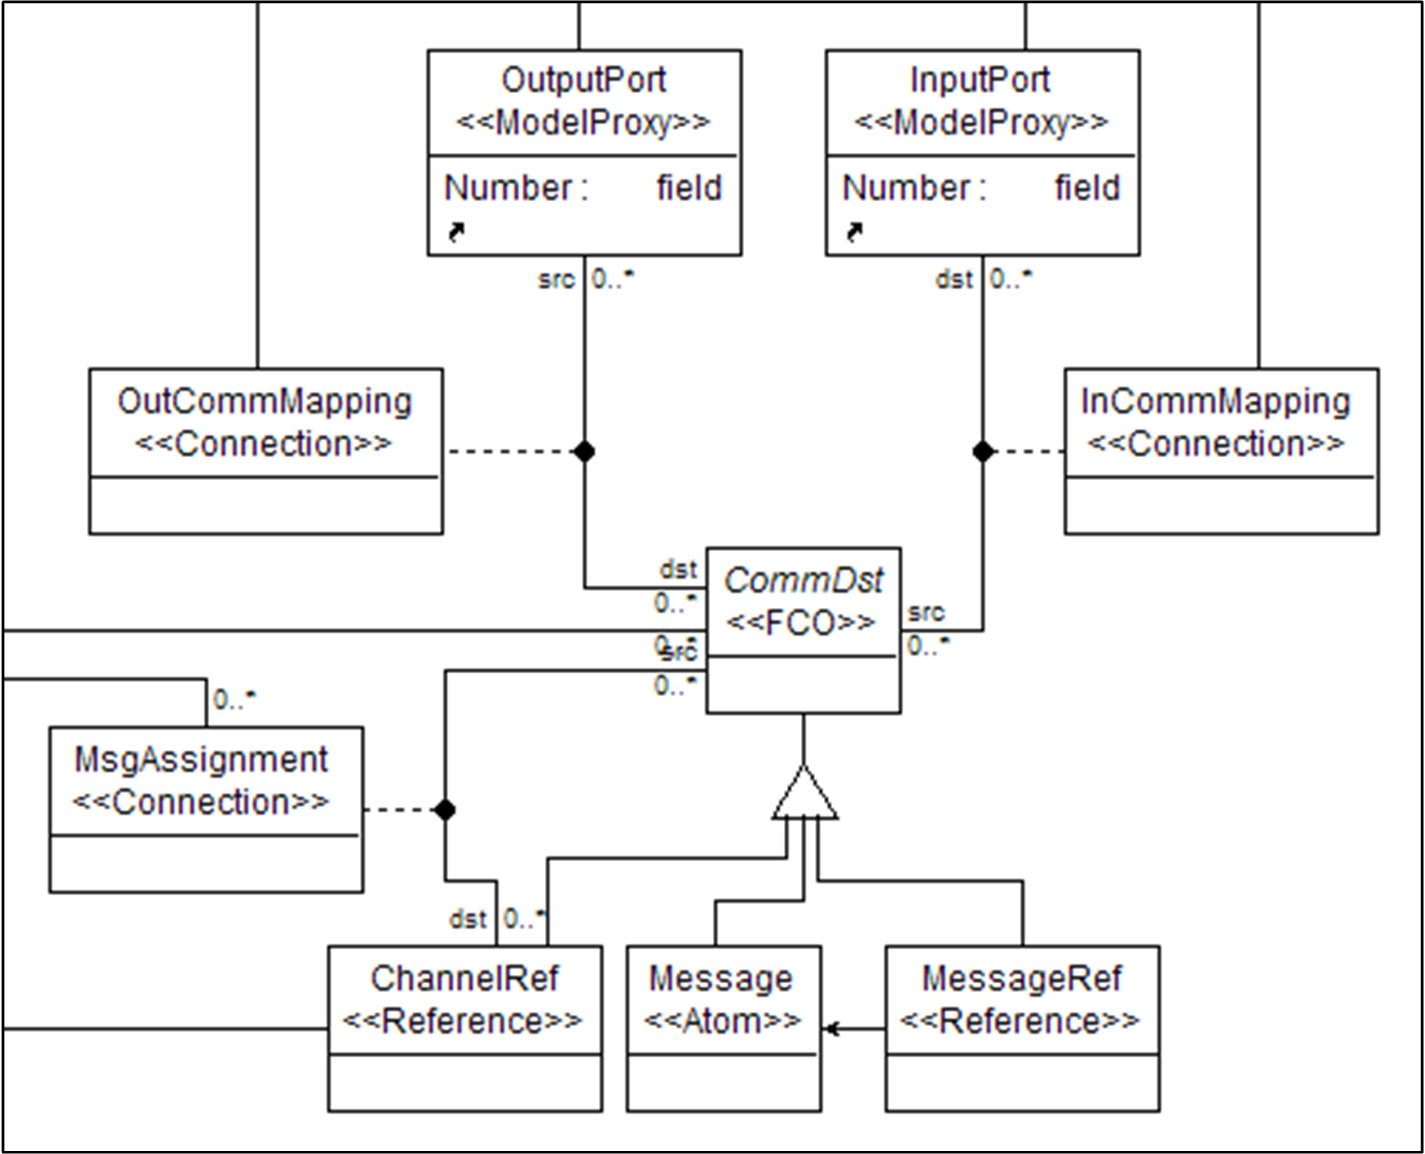
\includegraphics[width=0.9\columnwidth]{diagrams/depportnew.png}
%	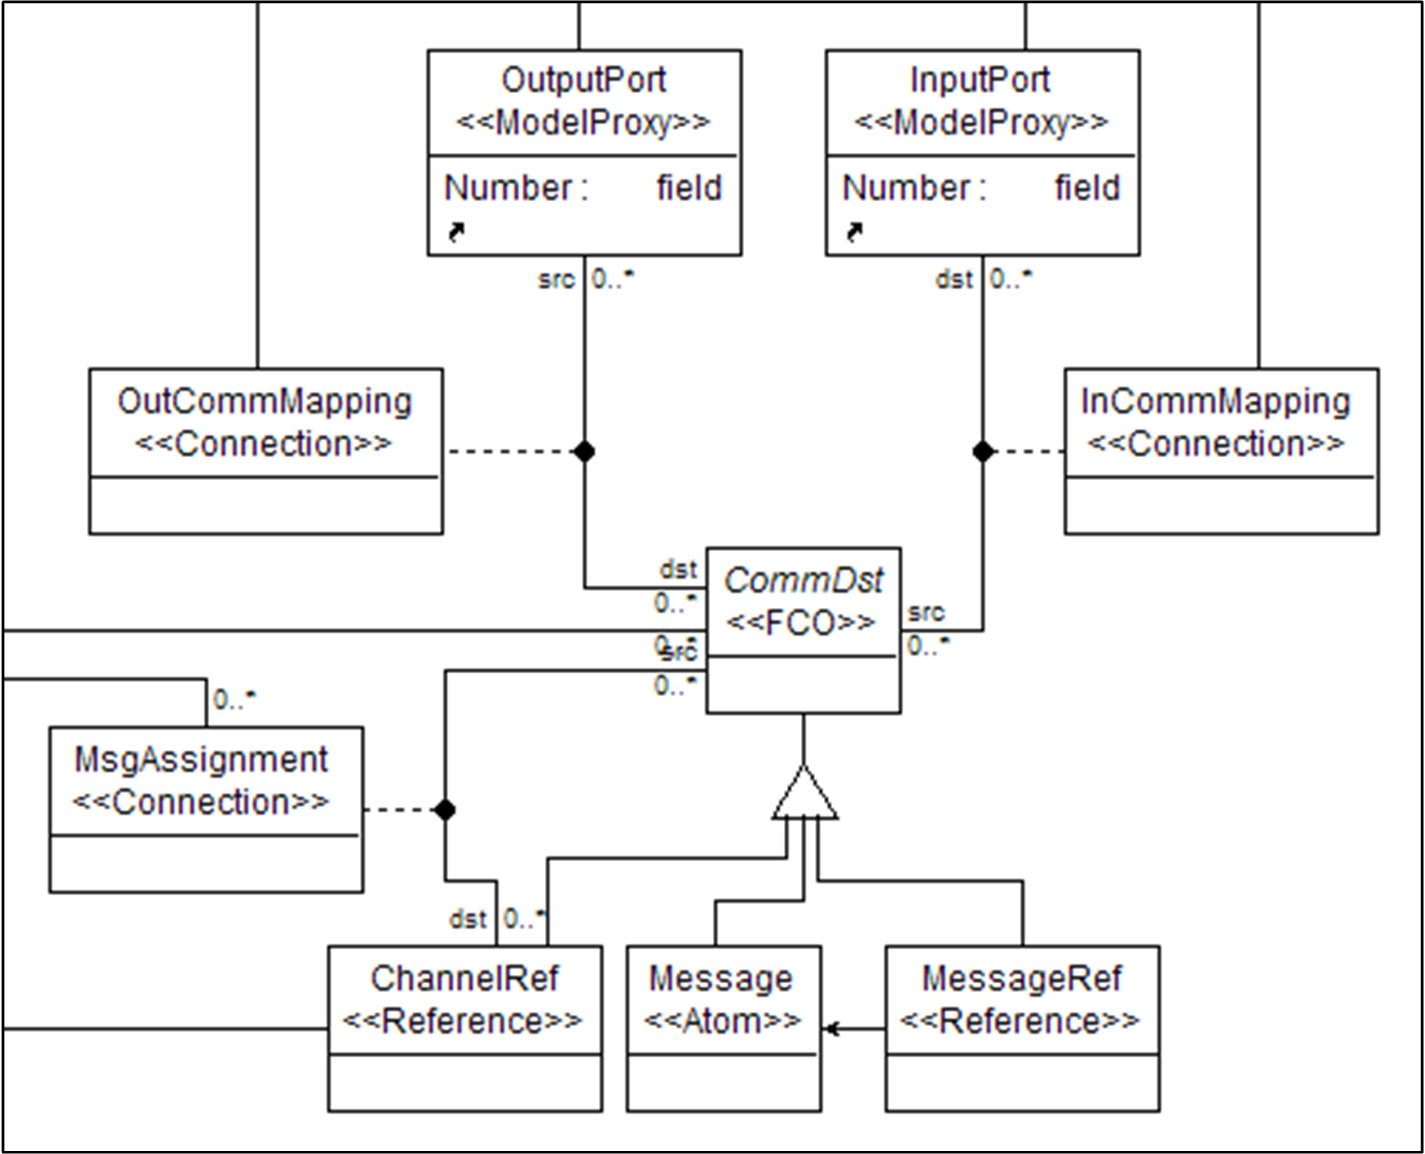
\includegraphics[scale=0.9]{diagrams/depportnew.png}
%	\label{fig:depport}
%	}
	\caption{Details from deployment sublanguage.}
	\label{fig:depnew}
\end{figure}

Similarly, Fig. \ref{fig:arch} describes the software architecture language. The Connector element models communication between components.  Semantic details of communication interactions remain abstract in this logical architecture -- the platform model must be specified and associated in order to completely specify the interactions (though in this version we only offer synchronous and time-triggered communications).

Deployment models capture the assignment of Components (and Ports) from the Architecture to Platform Nodes (and Channels).  Additional implementation details (e.g. worst-case execution time) are represented here for platform-specific synthesis.  Fig. \ref{fig:depnew} shows the relevant modeling concepts.  Simulink objects SLInputPort and SLOutputPort are assigned to Message objects, which represent the marshaling of data to be sent on a Bus.

%\subsection{Current and Future Work}

%Simulink/Stateflow model import and code generation are the most mature features of the toolchain, so the described features are fairly well supported.  Ongoing work extends the number of Simulink blocks which can be synthesized by the code generator, and adds the ability to import Matlab functions embedded in the Simulink designs.